\documentclass[../TDM3_courbe_app.tex]{subfiles}%

\begin{document}
\section[s]"1"{Entraînement d'une spationaute}

\noindent
\enonce{%
  \noindent
	\begin{minipage}{0.70\linewidth}
		Une spationaute doit subir différents tests d'aptitude aux vols spatiaux,
		notamment le test des accélérations. Pour cela, on l'installe dans une
		capsule de centre O, fixée au bout d'un bras métallique horizontal dont
		l'autre extrémité est rigidement liée à un arbre de rotation vertical $\D$.
		La longueur du bras est notée $L$. On assimilera la spationaute au point
		matériel S. \bigbreak
	\end{minipage}
	\hfill
	\begin{minipage}{0.25\linewidth}
		\begin{center}
			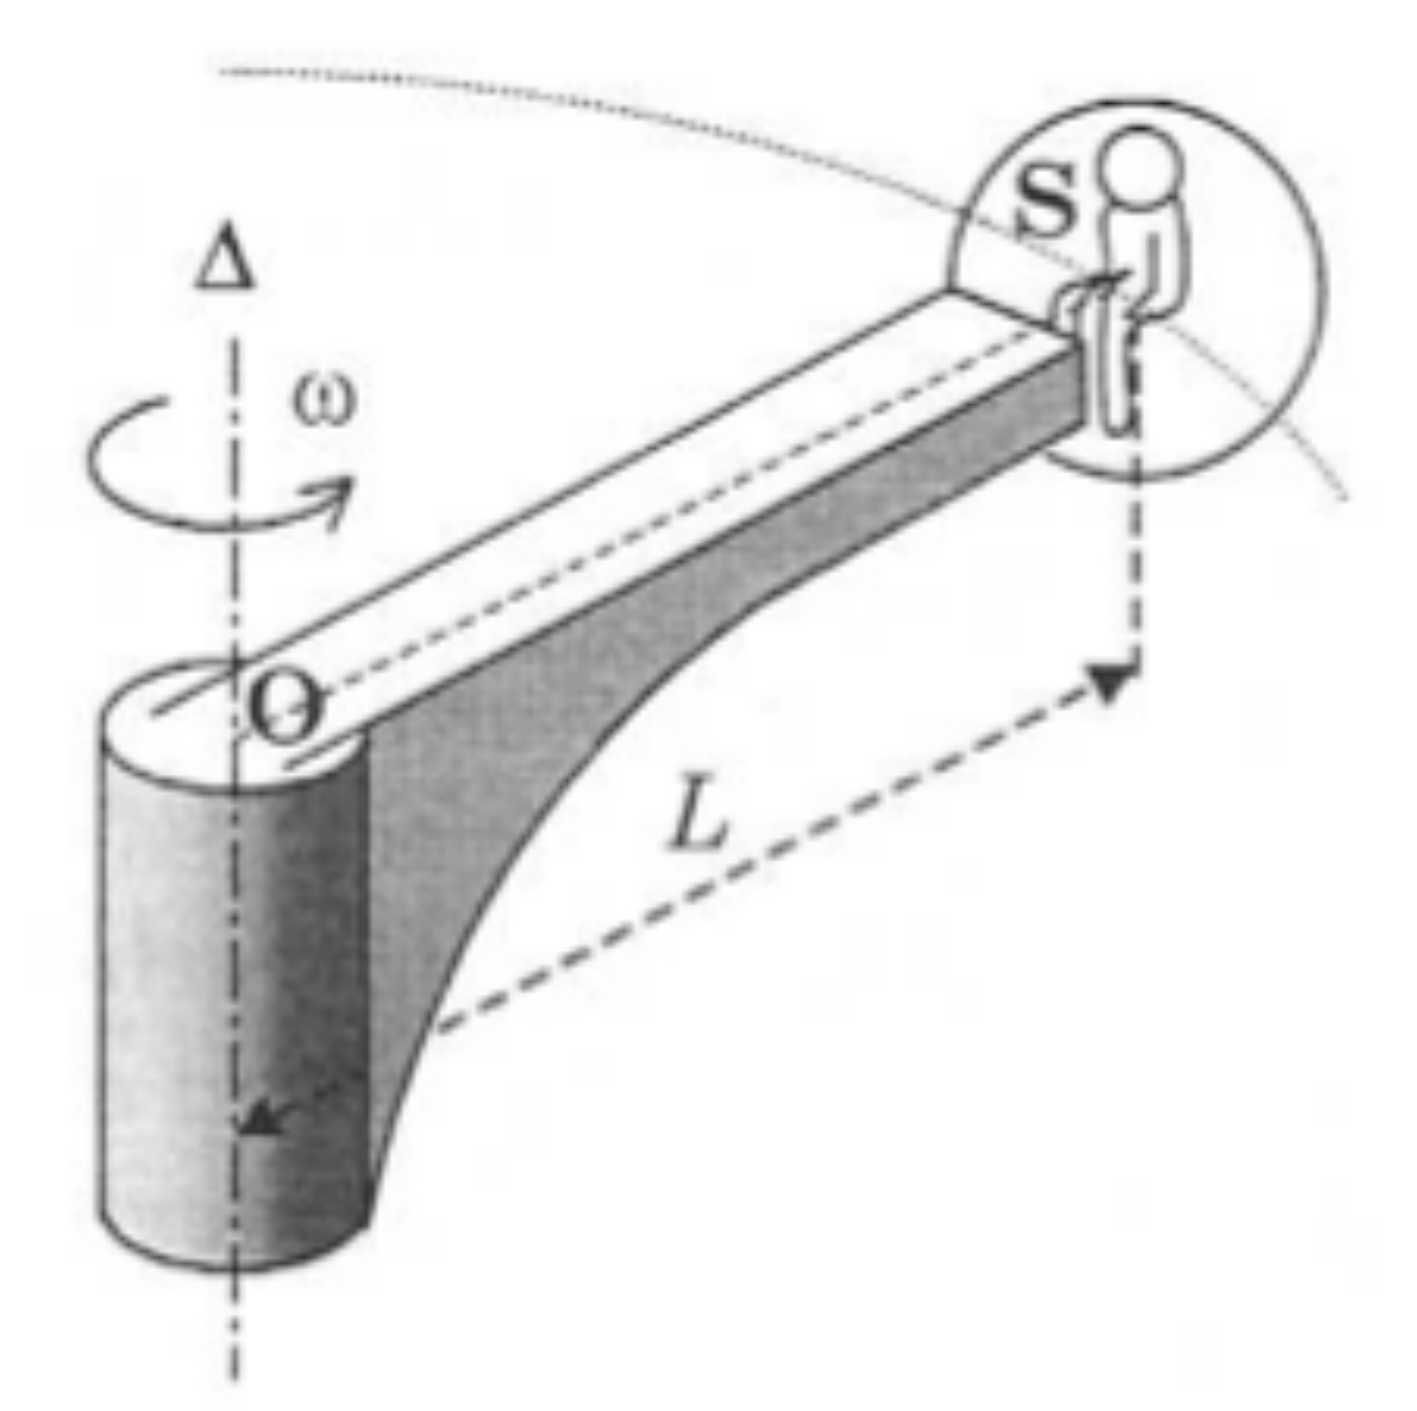
\includegraphics[width=\linewidth]{centri_spat-plain}
		\end{center}
	\end{minipage}
	L'ensemble \{capsule + bras + arbre\} est mis en rotation avec un vitesse
	angulaire croissant progressivement selon la loi
	\[\w(t) = \w_0(1-\exp^{-t/\tau})\]
	avec $\w_0$ la vitesse angulaire nominale du simulateur, et $\tau$ un temps
	caractéristique. On donne $L = \SI{10.0}{m}$ et $g = \SI{9.81}{m.s^{-2}}$.
}%

\QR{%
	Établir proprement le système d'étude.
}{%
  \leavevmode\vspace*{-15pt}\relax
	\begin{itemize}[label=$\diamond$] %, leftmargin=10pt]
		\item[b]{Système}~: \{spationaute\}
		\item[b]{Référentiel}~: référentiel du laboratoire, supposé galiléen
		\item[b]{Repère}~: $(\Or,\ur,\ut)$ avec $\ut$ selon le sens de rotation
	\end{itemize}
  \vspace{-35pt}
	\begin{minipage}{0.60\linewidth}
		\begin{itemize}[label=$\diamond$] %, leftmargin=10pt]
			\item[b]{Repérage}~:
			\begin{align*}
				\vv{\rm OS}(t) & = L\ur                   \\
				\vf_S(t)       & = L\w(t)\ut                 \\
				\af_S(t)       & = L\dot{\w}(t)\ut -L\w^2(t)\ur
			\end{align*}
		\end{itemize}
	\end{minipage}
	\hfill
	\begin{minipage}{0.35\linewidth}
		\begin{center}
			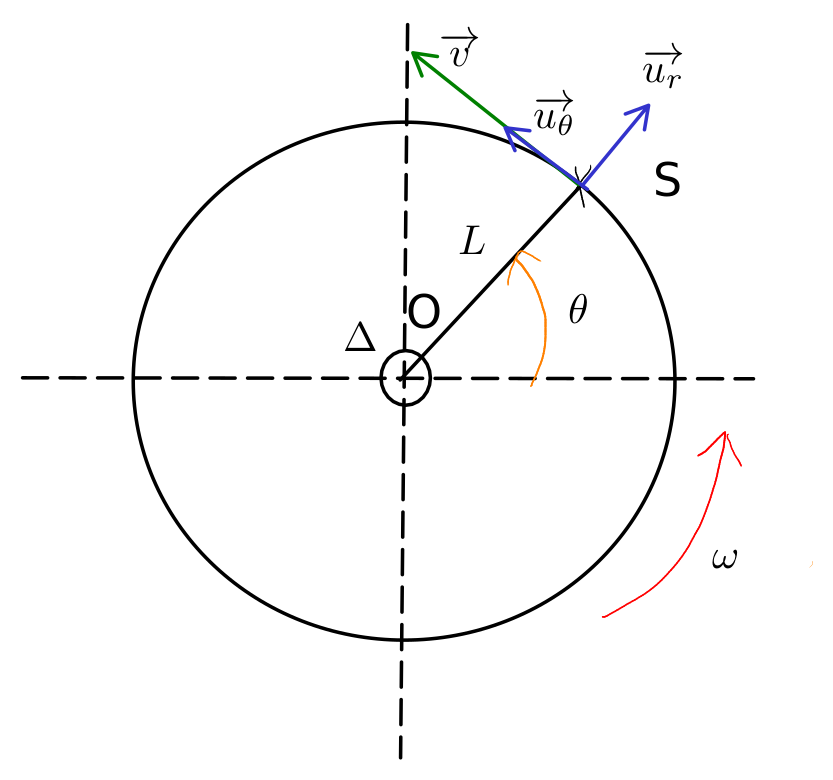
\includegraphics[scale=0.15]{spationaute_corr}
		\end{center}
	\end{minipage}
}
\QR{%
	À partir de quelle durée peut-on supposer que le mouvement est
	circulaire et uniforme~? Que deviennent les expressions des vecteurs
	vitesse et accélération dans ce cas~? Calculer alors la norme de
	l'accélération subie par la spationaute.
}{%
	Au bout de quelques $\tau$, $\w(t) = \w_0$ et le mouvement sera
	circulaire uniforme. Les vecteurs vitesse et accélération deviennent~:
	\begin{empheq}[box=\fbox, left=\empheqlbrace]{align*}
		\vf_S(t) &= L\w_0\ut\\
		\af_S(t) &= -L\w_0{}^2\ur
	\end{empheq}
	La norme de l'accélération subie est alors \fbox{$\norm{\af_S} =
			L\w_0{}^2$}.
}
\QR{%
	Quelle doit être la valeur de $\w_0$ pour que l'accélération atteigne
	\SI{10}{g} lors du régime de rotation uniforme~? On donnera le résultat
	en tours par second.
}{%
	\begin{gather}
		a_S = 10g \Ra \boxed{\w_0 = \sqrt{\frac{10g}{L}}}
		\qavec
		\left\{
		\begin{array}{rcl}
			g & = & \SI{9.81}{m.s^{-2}} \\
			L & = & \SI{10.0}{m}
		\end{array}
		\right.\\
		\AN
		\boxed{\w_0 = \SI{3.13}{rad.s^{-1}} \approx \SI{0.50}{tour.s^{-1}}}
	\end{gather}
	\begin{tcb}(odgr){}
		\begin{itemize}[label=$\diamond$]
			\item Accélération latérale en F1~: \SIrange{4}{5}{g}~;
			\item Accélération latérale en avion de chasse~: \SIrange{9}{10}{g}
			      pendant quelques secondes max~;
			\item Accélération verticale, éjection d'un avion de chasse~: $\approx
				      \SI{20}{g}$ (interdiction de vol après 2 utilisation du siège
			      éjectable à cause – notamment – du tassement des vertèbres)~;
			\item Accélération négative frontale en accident de voiture~:
			      \SIrange{40}{60}{g}~! Même sans choc physique, une telle
			      décélération cause des hémorragies internes à cause des organes
			      internes percutant les os. Soyez prudent-es.
		\end{itemize}
	\end{tcb}
}%
\end{document}
